\subsection{Session Execution Activity}

\begin{figure}[H]
    \centering
    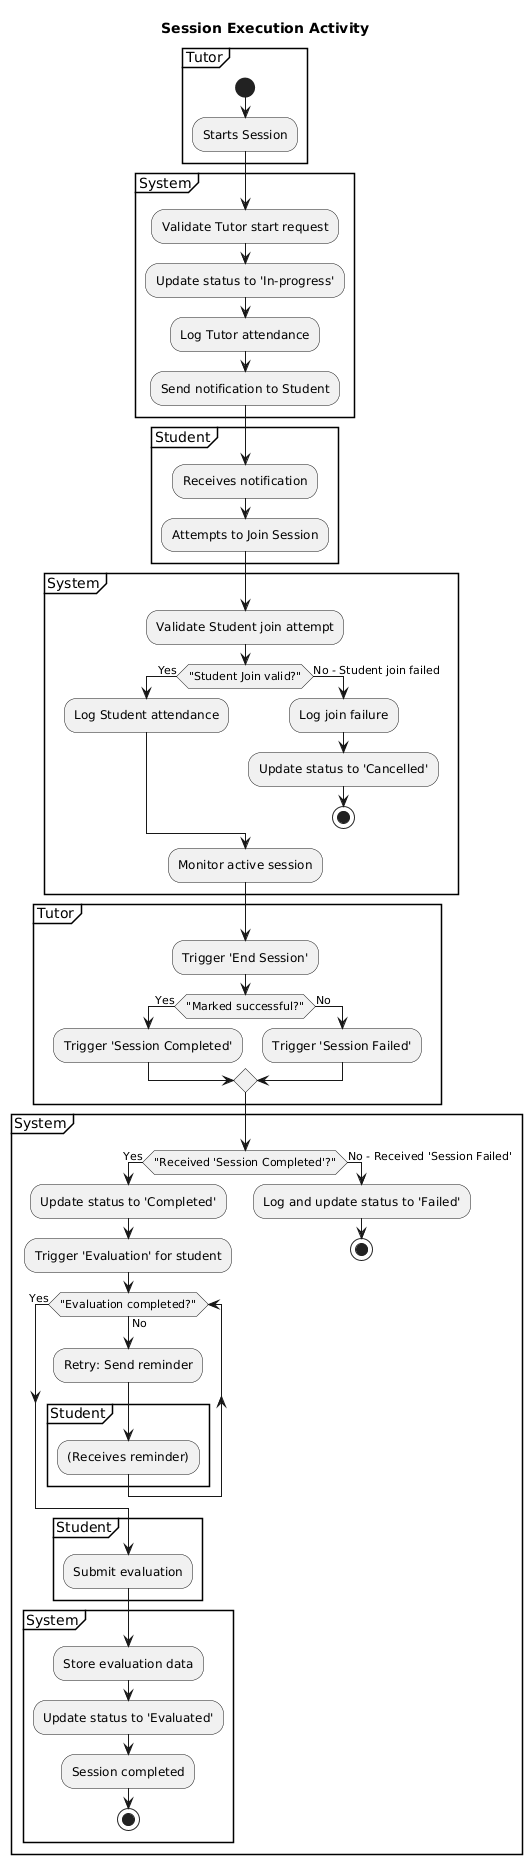
\includegraphics[width=0.35\textwidth]{graphics/chapter4/student/Session_Exc.png}
    \caption{Session Execution Process}
    \label{fig:Execute}
\end{figure}

\noindent \textbf{Description}
\begin{enumerate}
    \item \textbf{Tutor}: Start session and notifies the system.
    \item \textbf{System}: Validates request and updates status.
    \item \textbf{Student}: Receives notifications and joins.
    \item \textbf{System}: Validates join request.
    \item \textbf{System}: Student join valid?.
        \begin{enumerate}
            \item \textbf{Yes:} Log attendance and monitor the session.
            \item \textbf{No:} Log the join failure, update status and \textit{Flows end}.
        \end{enumerate}
    \item \textbf{Tutor}: End session and marked it.
   \item \textbf{Tutor}: Marked "Successful"?.
        \begin{enumerate}
            \item \textbf{Yes:} Trigger "Session Completed".
            \item \textbf{No:} Trigger "Session Failed" (due to Internet connection, etc).
        \end{enumerate}
    \item \textbf{Decision}: receive a "Session Completed" trigger?.
        \begin{enumerate}
            \item \textbf{Yes:} Updates status and triggers the 'Evaluation'.
            \item \textbf{No:} Logs the failure, updates status and \textit{Flows end}.
        \end{enumerate}
    \item \textbf{Student:} Receives evaluation reminders and submits the evaluation.
    \item \textbf{System:} Stores the evaluation data, updates the status and \textit{Flow ends.}
\end{enumerate}